探索の章で扱うアルゴリズムは以下と通りです。

\begin{itemize}
  \item 線形探索
  \item 二分探索
  \item 二分探索木
  \item Treeq
  \item 平衡木(AVL木、B木、赤黒木)
  \item ハッシュ法
\end{itemize}

検索(サーチ)とは、データ集合(配列など)から、目的とする値を持った要素を探し出すことを意味する。

\section{線形探索}

\textbf{線形探索}は、目的とする要素が見つかるまで先頭から順に要素を見ていく探索方法です。例えば、以下の配列で0を探すなら前から順番に、
8, 4, 5, 0, 2の順に要素を見ていきます。

\vspace{0.5cm}

\begin{center}
  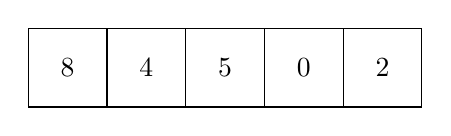
\begin{tikzpicture}
      \draw (0, 0) rectangle (1, 1);
      \node at (0.5, 0.5) {8};
      
      \draw (1, 0) rectangle (2, 1);
      \node at (1.5, 0.5) {4};
      
      \draw (2, 0) rectangle (3, 1);
      \node at (2.5, 0.5) {5};
      
      \draw (3, 0) rectangle (4, 1);
      \node at (3.5, 0.5) {0};
      
      \draw (4, 0) rectangle (5, 1);
      \node at (4.5, 0.5) {2};
  \end{tikzpicture}
\end{center}

\subsection{線形探索の実装}
\begin{lstlisting}[caption=線形探索の実装, frame=TRBL, label={linear}]
def linear_search(array: list[int], value: int) -> int:
    """
    線形探索をして一致するならそのindexを返す. 一致しないときは-1を返す
    """
    for i in range(len(array)):
        if array[i] == value:
            return i
    
    return -1


\end{lstlisting}

\subsection{番兵}

番兵法では探索するデータ集合の最後に目的とする数を追加します。最後に番兵を追加することで、より効率的に探索を行うことができます。
実際には番兵を追加してもそこまで効率が良くなるわけではないですが、番兵を追加することで、ループの条件判定を省略することができます。

\vspace{0.5cm}

\begin{center}
  \begin{tikzpicture}
      \draw (0, 0) rectangle (1, 1);
      \node at (0.5, 0.5) {8};
      
      \draw (1, 0) rectangle (2, 1);
      \node at (1.5, 0.5) {4};
      
      \draw (2, 0) rectangle (3, 1);
      \node at (2.5, 0.5) {5};
      
      \draw (3, 0) rectangle (4, 1);
      \node at (3.5, 0.5) {3};
      
      \draw (4, 0) rectangle (5, 1);
      \node at (4.5, 0.5) {2};
      
      \draw (5, 0) rectangle (6, 1);
      \fill[red, overlay] (5, 0) rectangle (6, 1);
      \node[white] at (5.5, 0.5) {0};
      \node[] at (5.5, -0.5) {番兵};
  \end{tikzpicture}
\end{center}

\begin{lstlisting}[caption=番兵の実装, frame=TRBL, label={sentinel}]
def linear_search(array: list[int], value: int) -> int:
    """
    線形探索をして一致するならそのindexを返す. 一致しないときは-1を返す
    """
    i = 0
    copied_array = array.copy()
    copied_array.append(value)
    while copied_array[i] != value: i += 1
    
    return i if i < len(array) else -1
  \end{lstlisting}

\section{二分探索}

\subsection{配列を探索する二分探索}

二分探索はソートされた配列に対して高速に探索を行うアルゴリズムの一つです。二分探索では探索する区間が条件に応じてどんどん半分になっていくため、
計算量は$O(\log n)$となります。以下の配列に対して、二分探索で18を探す場合を考えましょう。

最初の区間は配列全体を取ります。0-indexedな配列を考えると、midは39となり目的の18より大きいです。midが目的の値より大きい場合、
右の区間を狭めます。right = mid - 1とします。

\vspace{0.5cm}

\begin{center}
  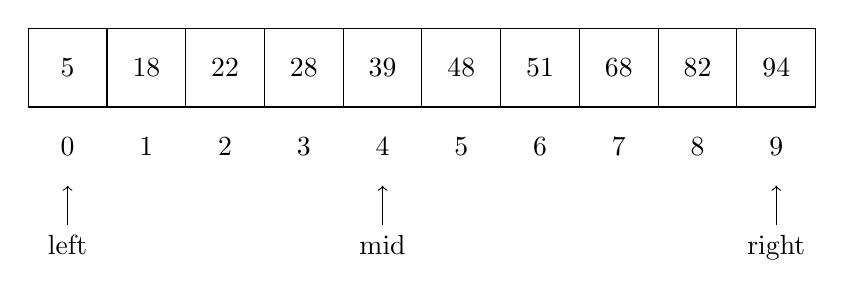
\begin{tikzpicture}
      \draw (0, 0) rectangle (1, 1);
      \node at (0.5, 0.5) {5};
      
      \draw (1, 0) rectangle (2, 1);
      \node at (1.5, 0.5) {18};
      
      \draw (2, 0) rectangle (3, 1);
      \node at (2.5, 0.5) {22};
      
      \draw (3, 0) rectangle (4, 1);
      \node at (3.5, 0.5) {28};
      
      \draw (4, 0) rectangle (5, 1);
      \node at (4.5, 0.5) {39};
      
      \draw (5, 0) rectangle (6, 1);
      \node at (5.5, 0.5) {48};
      
      \draw (6, 0) rectangle (7, 1);
      \node at (6.5, 0.5) {51};
      
      \draw (7, 0) rectangle (8, 1);
      \node at (7.5, 0.5) {68};
      
      \draw (8, 0) rectangle (9, 1);
      \node at (8.5, 0.5) {82};
      
      \draw (9, 0) rectangle (10, 1);
      \node at (9.5, 0.5) {94};

      \foreach \i in {0,1,...,9} {
        \node at (\i+0.5, -0.5) {\i};
    }

      % ラベルをはる
      \draw[<-] (0.5, -1) -- (0.5, -1.5) node[below] {left};
      \draw[<-] (9.5, -1) -- (9.5, -1.5) node[below] {right};
      \draw[<-] (4.5, -1) -- (4.5, -1.5) node[below] {mid};
  \end{tikzpicture}
\end{center}

\vspace{0.5cm}

rightを3に更新しました。mid = (0 + 3) // 2 = 1となります。midの値は18で目的の値と一致します。

\vspace{0.5cm}

\begin{center}
  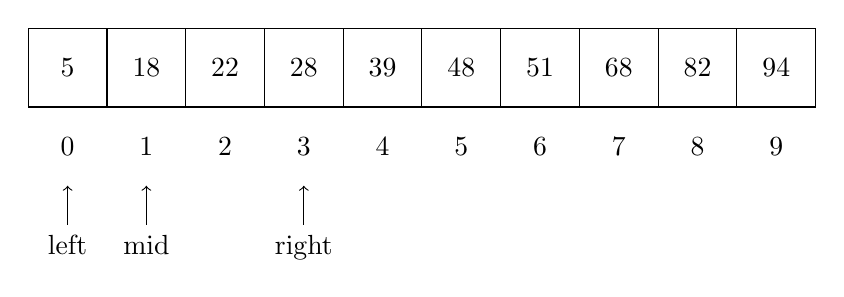
\begin{tikzpicture}
      \draw (0, 0) rectangle (1, 1);
      \node at (0.5, 0.5) {5};
      
      \draw (1, 0) rectangle (2, 1);
      \node at (1.5, 0.5) {18};
      
      \draw (2, 0) rectangle (3, 1);
      \node at (2.5, 0.5) {22};
      
      \draw (3, 0) rectangle (4, 1);
      \node at (3.5, 0.5) {28};
      
      \draw (4, 0) rectangle (5, 1);
      \node at (4.5, 0.5) {39};
      
      \draw (5, 0) rectangle (6, 1);
      \node at (5.5, 0.5) {48};
      
      \draw (6, 0) rectangle (7, 1);
      \node at (6.5, 0.5) {51};
      
      \draw (7, 0) rectangle (8, 1);
      \node at (7.5, 0.5) {68};
      
      \draw (8, 0) rectangle (9, 1);
      \node at (8.5, 0.5) {82};
      
      \draw (9, 0) rectangle (10, 1);
      \node at (9.5, 0.5) {94};

      \foreach \i in {0,1,...,9} {
        \node at (\i+0.5, -0.5) {\i};
    }

      % ラベルをはる
      \draw[<-] (0.5, -1) -- (0.5, -1.5) node[below] {left};
      \draw[<-] (1.5, -1) -- (1.5, -1.5) node[below] {mid};
      \draw[<-] (3.5, -1) -- (3.5, -1.5) node[below] {right};
  \end{tikzpicture}
\end{center}

\vspace{0.5cm}

次に、目的とする値を19として配列に存在しない場合を考えましょう。mid = 1の値は18で目的の値よりも小さいので、下の図のようにleftをmid + 1に更新します。
mid = (2 + 3) // 2 = 2となります。midの値は22で目的の値より大きいです。よって、rightをmid - 1に更新します。
すると、right = 1, left = 2となり、left > rightとなるので探索を終了します。

\vspace{0.5cm}

\begin{center}
  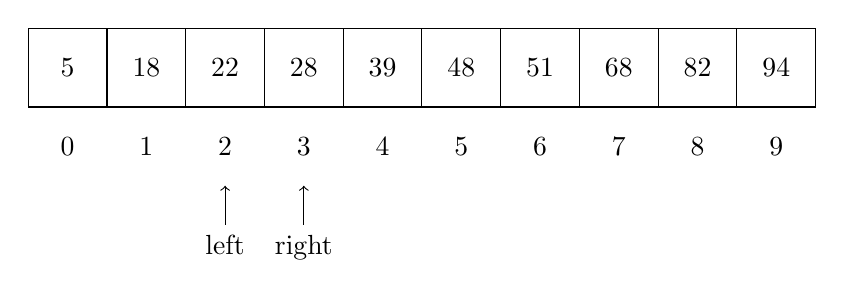
\begin{tikzpicture}
      \draw (0, 0) rectangle (1, 1);
      \node at (0.5, 0.5) {5};
      
      \draw (1, 0) rectangle (2, 1);
      \node at (1.5, 0.5) {18};
      
      \draw (2, 0) rectangle (3, 1);
      \node at (2.5, 0.5) {22};
      
      \draw (3, 0) rectangle (4, 1);
      \node at (3.5, 0.5) {28};
      
      \draw (4, 0) rectangle (5, 1);
      \node at (4.5, 0.5) {39};
      
      \draw (5, 0) rectangle (6, 1);
      \node at (5.5, 0.5) {48};
      
      \draw (6, 0) rectangle (7, 1);
      \node at (6.5, 0.5) {51};
      
      \draw (7, 0) rectangle (8, 1);
      \node at (7.5, 0.5) {68};
      
      \draw (8, 0) rectangle (9, 1);
      \node at (8.5, 0.5) {82};
      
      \draw (9, 0) rectangle (10, 1);
      \node at (9.5, 0.5) {94};

      \foreach \i in {0,1,...,9} {
        \node at (\i+0.5, -0.5) {\i};
    }

      % ラベルをはる
      \draw[<-] (2.5, -1) -- (2.5, -1.5) node[below] {left};
      \draw[<-] (3.5, -1) -- (3.5, -1.5) node[below] {right};
  \end{tikzpicture}
\end{center}

二分探索の実装は以下の通りです。

\begin{lstlisting}[caption=二分探索の実装, frame=TRBL, label={simle_binary}]
def binary_search(A: list[int], value: int) -> int:
    left, right = 0, len(A) - 1
    
    while left <= right:
        mid = (left + right) // 2
        
        if A[mid] == value:
            return mid
        
        if A[mid] < value:
            left = mid + 1
        else:
            right = mid - 1
    
    return -1
\end{lstlisting}

\subsection{一般化した二分探索}
Pythonの標準ライブラリであるbisectのbisect\_leftの実装をしましょう。bisect\_leftはソートされた配列に対して、
与えられた値以上の最小のindexを返す関数です。bisect\_leftは二分探索を用いて実装されています。先ほどの配列から要素を探す二分探索では、要素一致するか否かを判定していましたが、
今回はもっと一般化して「midがある条件を満たすか否か」を判定して範囲を狭めていきます。このとき、leftより右側の区間は
条件を満たさず、rightより左側の区間は条件を満たすようにします。 

二分探索では以下の図のような条件を満たす赤い部分を条件を満たす境界ギリギリになるように更新していきます。

\begin{itemize}
  \item leftは常に条件を満たさない
  \item rightは常に条件を満たす
\end{itemize}

という条件を満たすように処理を進めていき、最終的にleftが条件を満たさない最大のindex、rightが条件を満たす最小のindexを返します。
bisect\_leftではleftが与えられた値よりも小さく、rightが与えられた値以上の最小のindexを返す関数です。

\vspace{0.5cm}

\begin{center}
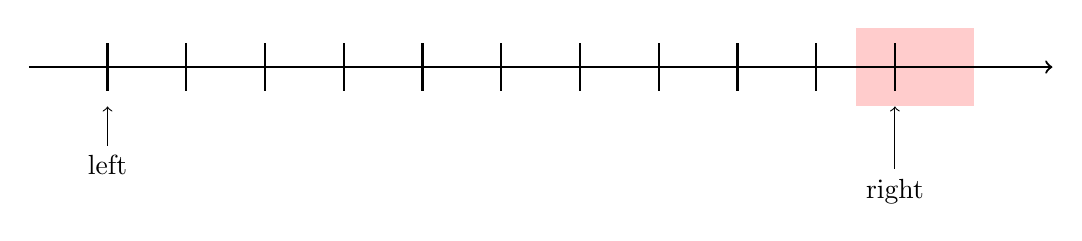
\begin{tikzpicture}
    \fill[red!20] (10.5, 0.5) rectangle (12, 1.5);
    \foreach \x in {1, 2, 3, 4, 5, 6, 7, 8, 9, 10, 11} {
        \draw[thick] (\x, 0.7) -- (\x, 1.3);
    }

    \draw[->, thick] (0, 1) -- (13, 1);
    \draw[<-] (1, 0.5) -- (1, -0.) node[below] {left};
    \draw[<-] (11, 0.5) -- (11, -0.3) node[below] {right};
\end{tikzpicture}
\end{center}

\begin{center}
  \textbf{初期状態}
\end{center}

\vspace{0.5cm}

\begin{center}
  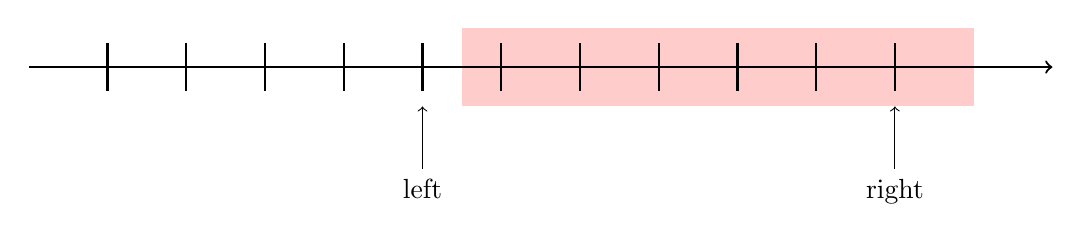
\begin{tikzpicture}
      \fill[red!20] (5.5, 0.5) rectangle (12, 1.5);
      \foreach \x in {1, 2, 3, 4, 5, 6, 7, 8, 9, 10, 11} {
          \draw[thick] (\x, 0.7) -- (\x, 1.3);
      }
  
      \draw[->, thick] (0, 1) -- (13, 1);
      \draw[<-] (5, 0.5) -- (5, -0.3) node[below] {left};
      \draw[<-] (11, 0.5) -- (11, -0.3) node[below] {right};
  \end{tikzpicture}
  \end{center}
  
  \begin{center}
    \textbf{終了状態}
  \end{center}

bisect\_leftの実装は以下の通りです。

\begin{lstlisting}[caption=bisect\_leftの実装, frame=TRBL, label={bisect_left}]
def bisect_left(array: list[int], key: int) -> int:
  left, right = -1, len(array)
  
  while right - left > 1:
      mid = (left + right) // 2
      
      if array[mid] < key:
          left = mid
      else:
          right = mid
  
  return right
\end{lstlisting}

bisect\_leftの実装では、左側が条件を満たさない、右側が条件を満たすといった実装になっています。これだとまだ条件次第でleftが条件を満たす、rightが条件を満たさないという
実装もあり得ます。そこで以下ではめぐる式二分探索のさらに一般化した実装を紹介します。

\subsection{めぐる式二分探索}

めぐる式二分探索では、

\begin{itemize}
  \item ngは常に条件を満たさない
  \item okは常に条件を満たす
\end{itemize}

のように数直線上の右や左という概念を持たせずに実装します。めぐる式二分探索は以下のように実装されます。
is\_okは条件を満たすかどうかを判定する関数ですので、条件に合わせて実装します。

\begin{lstlisting}[caption=めぐる式二分探索, frame=TRBL, label={megru}]
def binary_search(array: list[int], key: int):
    ng, ok = -1, len(array)
    
    while abs(ok - ng) > 1:
        mid = (ng + ok) // 2
        
        if is_ok(array, mid, key):
            ok = mid
        else:
            ng = mid
    
    return ok
\end{lstlisting}

\newpage

\section{二分探索木}
二分探索は探索自体は$O(\log n)$で行うことができますが、配列がソートされているひつようがあり、データの挿入や削除がある場合は毎回ソートがあり非効率ではあります。
解決策としては、\textbf{データ構造で解決}や\textbf{Treeq}などがあります。データ構造で解決する方法の一つが\textbf{二分探索木}です。

\textbf{二分探索木}は以下の性質を持った木構造です。

\begin{itemize}
  \item 左子ノードは親ノードよりも小さい(または等しい) (下の図では$B \leq A$)
  \item 右子ノードは親ノードよりも大きい (下の図では$A < C$)
\end{itemize}

\begin{center}
    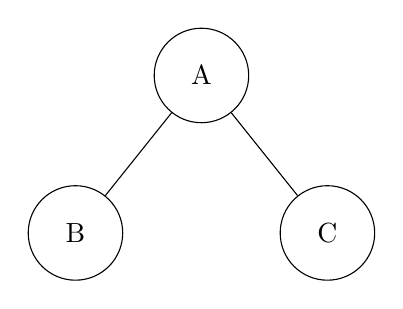
\begin{tikzpicture}[scale=0.4]
      \node[circle, draw, minimum size=1.2cm] (A) at (0, 0) {};
      \node[circle, draw, minimum size=1.2cm] (B) at (-4, -5) {};
      \node[circle, draw, minimum size=1.2cm] (C) at (4, -5) {};

      % 線を引く
      \draw (A) --(B);
      \draw (A) -- (C);

      % 値を入れる
      \node at (0, 0) {A};
      \node at (-4, -5) {B};
      \node at (4, -5) {C};
    \end{tikzpicture}
\end{center}

二分探索木で行う処理は以下の通りです。

\begin{itemize}
  \item 木の作成
  \item 探索
  \item 削除
\end{itemize}

\subsection{二分探索木の作成}
\texttt{[22,18, 5, 82, 51, 39]}の配列を二分探索木に変換してみましょう。

\vspace{0.5cm}

\begin{center}
  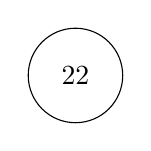
\begin{tikzpicture}
    \node[circle, draw, minimum size=1.2cm] (A) at (0, 0) {}; 

    % 値を入れる
    \node at (0, 0) {22};
  \end{tikzpicture}
\end{center}

\begin{center}
  \textbf{22を挿入}
\end{center}

\vspace{0.5cm}

\begin{center}
  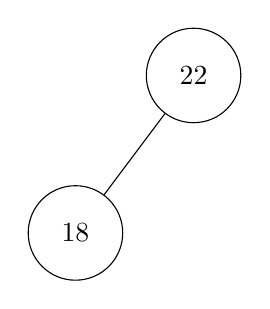
\begin{tikzpicture}
    \node[circle, draw, minimum size=1.2cm] (A) at (0, 0) {}; 
    \node[circle, draw, minimum size=1.2cm] (B) at (-1.5, -2) {};

    % 線を引く
    \draw (A) --(B);

    % 値を入れる
    \node at (0, 0) {22};
    \node at (-1.5, -2) {18};
  \end{tikzpicture}
\end{center}

\begin{center}
  \textbf{18を挿入}
\end{center}

\vspace{0.5cm}

\begin{center}
  \begin{tikzpicture}
    \node[circle, draw, minimum size=1.2cm] (A) at (0, 0) {}; 
    \node[circle, draw, minimum size=1.2cm] (B) at (-1.5, -2) {};
    \node[circle, draw, minimum size=1.2cm] (C) at (-3, -4) {};

    % 線を引く
    \draw (A) --(B);
    \draw (B) -- (C);

    % 値を入れる
    \node at (0, 0) {22};
    \node at (-1.5, -2) {18};
    \node at (-3, -4) {5};
  \end{tikzpicture}
\end{center}

\begin{center}
  \textbf{5を挿入}
\end{center}

\vspace{0.5cm}

\begin{center}
  \begin{tikzpicture}
    \node[circle, draw, minimum size=1.2cm] (A) at (0, 0) {}; 
    \node[circle, draw, minimum size=1.2cm] (B) at (-1.5, -2) {};
    \node[circle, draw, minimum size=1.2cm] (C) at (-3, -4) {};
    \node[circle, draw, minimum size=1.2cm] (D) at (1.5, -2) {};

    % 線を引く
    \draw (A) --(B);
    \draw (B) -- (C);
    \draw (A) -- (D);

    % 値を入れる
    \node at (0, 0) {22};
    \node at (-1.5, -2) {18};
    \node at (-3, -4) {5};
    \node at (1.5, -2) {82};
  \end{tikzpicture}
\end{center}

\begin{center}
  \textbf{82を挿入}
\end{center}

\vspace{0.5cm}

\begin{center}
  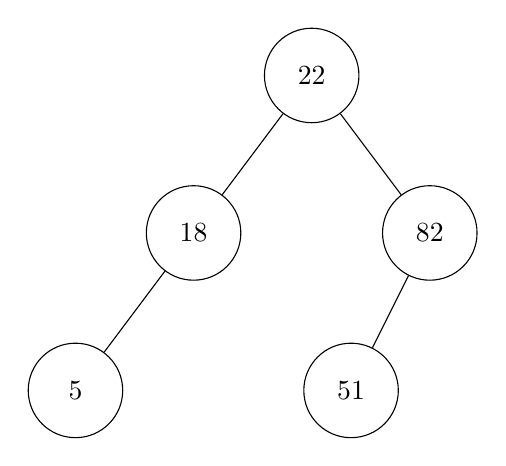
\begin{tikzpicture}
    \node[circle, draw, minimum size=1.2cm] (A) at (0, 0) {}; 
    \node[circle, draw, minimum size=1.2cm] (B) at (-1.5, -2) {};
    \node[circle, draw, minimum size=1.2cm] (C) at (-3, -4) {};
    \node[circle, draw, minimum size=1.2cm] (D) at (1.5, -2) {};
    \node[circle, draw, minimum size=1.2cm] (E) at (0.5, -4) {};

    % 線を引く
    \draw (A) --(B);
    \draw (B) -- (C);
    \draw (A) -- (D);
    \draw (D) -- (E);

    % 値を入れる
    \node at (0, 0) {22};
    \node at (-1.5, -2) {18};
    \node at (-3, -4) {5};
    \node at (1.5, -2) {82};
    \node at (0.5, -4) {51};
  \end{tikzpicture}
\end{center}

\begin{center}
  \textbf{51を挿入}
\end{center}

\vspace{0.5cm}

\begin{center}
  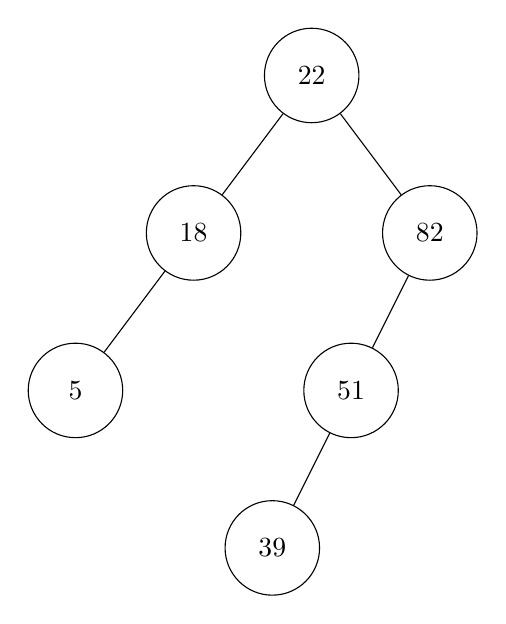
\begin{tikzpicture}
    \node[circle, draw, minimum size=1.2cm] (A) at (0, 0) {}; 
    \node[circle, draw, minimum size=1.2cm] (B) at (-1.5, -2) {};
    \node[circle, draw, minimum size=1.2cm] (C) at (-3, -4) {};
    \node[circle, draw, minimum size=1.2cm] (D) at (1.5, -2) {};
    \node[circle, draw, minimum size=1.2cm] (E) at (0.5, -4) {};
    \node[circle, draw, minimum size=1.2cm] (F) at (-0.5, -6) {};

    % 線を引く
    \draw (A) --(B);
    \draw (B) -- (C);
    \draw (A) -- (D);
    \draw (D) -- (E);
    \draw (E) -- (F);

    % 値を入れる
    \node at (0, 0) {22};
    \node at (-1.5, -2) {18};
    \node at (-3, -4) {5};
    \node at (1.5, -2) {82};
    \node at (0.5, -4) {51}; 
    \node at (-0.5, -6) {39};

  \end{tikzpicture}
\end{center}

\begin{center}
  \textbf{39を挿入}
\end{center}

\subsection{二分探索木の探索}
上の木を例に51を探してみましょう。根から順に探していきます。
\vspace{0.5cm}

\begin{center}
  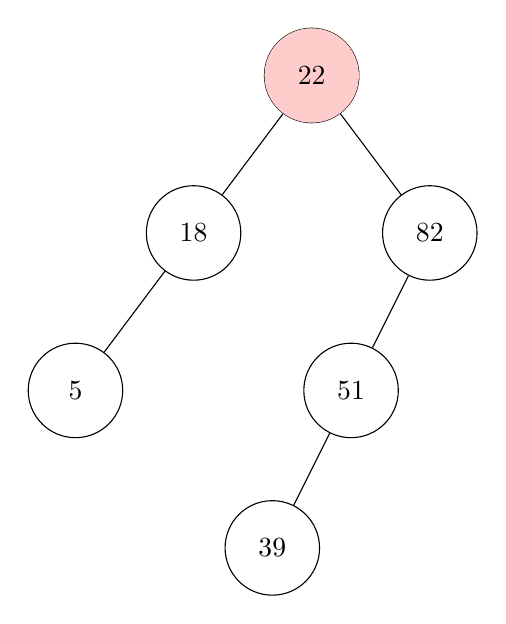
\begin{tikzpicture}
    \node[circle, draw, minimum size=1.2cm] (A) at (0, 0) {}; 
    \node[circle, draw, minimum size=1.2cm] (B) at (-1.5, -2) {};
    \node[circle, draw, minimum size=1.2cm] (C) at (-3, -4) {};
    \node[circle, draw, minimum size=1.2cm] (D) at (1.5, -2) {};
    \node[circle, draw, minimum size=1.2cm] (E) at (0.5, -4) {};
    \node[circle, draw, minimum size=1.2cm] (F) at (-0.5, -6) {};

    % 色を塗る
    \fill[red!20] (0, 0) circle (0.6);

    % 線を引く
    \draw (A) --(B);
    \draw (B) -- (C);
    \draw (A) -- (D);
    \draw (D) -- (E);
    \draw (E) -- (F);

    % 値を入れる
    \node at (0, 0) {22};
    \node at (-1.5, -2) {18};
    \node at (-3, -4) {5};
    \node at (1.5, -2) {82};
    \node at (0.5, -4) {51}; 
    \node at (-0.5, -6) {39};

  \end{tikzpicture}
\end{center}

\vspace{0.5cm}

51は22よりも大きいので右の子ノードに進みます。

\begin{center}
  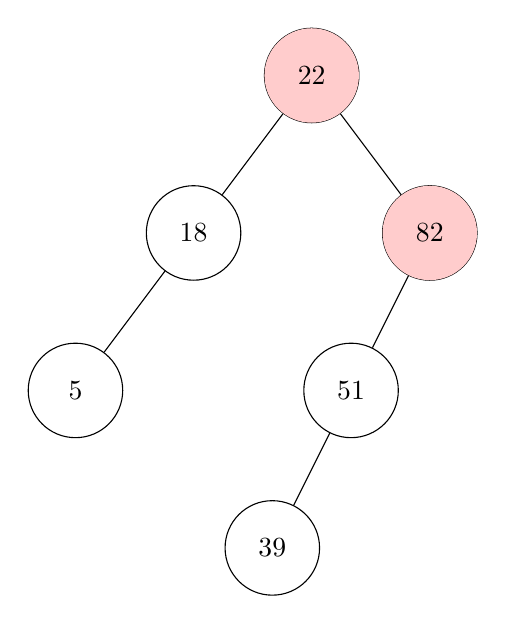
\begin{tikzpicture}
    \node[circle, draw, minimum size=1.2cm] (A) at (0, 0) {}; 
    \node[circle, draw, minimum size=1.2cm] (B) at (-1.5, -2) {};
    \node[circle, draw, minimum size=1.2cm] (C) at (-3, -4) {};
    \node[circle, draw, minimum size=1.2cm] (D) at (1.5, -2) {};
    \node[circle, draw, minimum size=1.2cm] (E) at (0.5, -4) {};
    \node[circle, draw, minimum size=1.2cm] (F) at (-0.5, -6) {};

    % 色を塗る
    \fill[red!20] (0, 0) circle (0.6);
    \fill[red!20] (1.5, -2) circle (0.6);

    % 線を引く
    \draw (A) --(B);
    \draw (B) -- (C);
    \draw (A) -- (D);
    \draw (D) -- (E);
    \draw (E) -- (F);

    % 値を入れる
    \node at (0, 0) {22};
    \node at (-1.5, -2) {18};
    \node at (-3, -4) {5};
    \node at (1.5, -2) {82};
    \node at (0.5, -4) {51}; 
    \node at (-0.5, -6) {39};

  \end{tikzpicture}
\end{center}

51は82よりも小さいので左の子ノードに進みます。見つかりました。

\vspace{0.5cm}

\begin{center}
  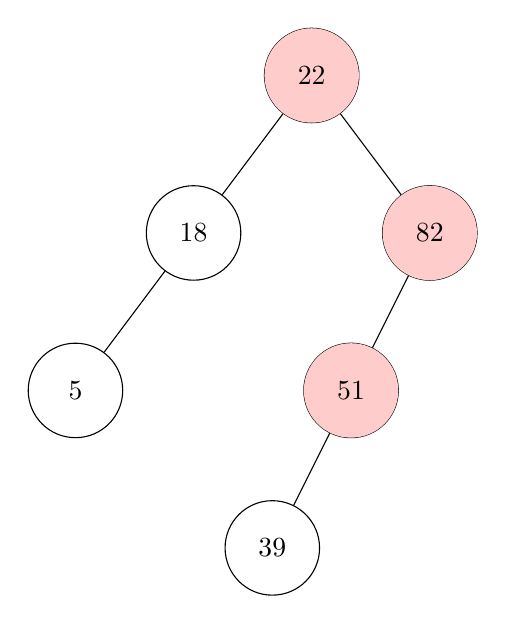
\begin{tikzpicture}
    \node[circle, draw, minimum size=1.2cm] (A) at (0, 0) {}; 
    \node[circle, draw, minimum size=1.2cm] (B) at (-1.5, -2) {};
    \node[circle, draw, minimum size=1.2cm] (C) at (-3, -4) {};
    \node[circle, draw, minimum size=1.2cm] (D) at (1.5, -2) {};
    \node[circle, draw, minimum size=1.2cm] (E) at (0.5, -4) {};
    \node[circle, draw, minimum size=1.2cm] (F) at (-0.5, -6) {};

    % 色を塗る
    \fill[red!20] (0, 0) circle (0.6);
    \fill[red!20] (1.5, -2) circle (0.6);
    \fill[red!20] (0.5, -4) circle (0.6);

    % 線を引く
    \draw (A) --(B);
    \draw (B) -- (C);
    \draw (A) -- (D);
    \draw (D) -- (E);
    \draw (E) -- (F);

    % 値を入れる
    \node at (0, 0) {22};
    \node at (-1.5, -2) {18};
    \node at (-3, -4) {5};
    \node at (1.5, -2) {82};
    \node at (0.5, -4) {51}; 
    \node at (-0.5, -6) {39};

  \end{tikzpicture}
\end{center}

\subsection{二分探索木の削除}

二分探索木からノードを削除する場合は以下の3つのケースがあります。

\begin{itemize}
  \item 子ノードがない場合
  \item 子ノードが1つの場合
  \item 子ノードが2つの場合
\end{itemize}

\subsubsection{子ノードがない場合}
例えば5を削除する場合を考えます。5は左右の子ノードがないので、他のノードに影響がないためそのまま削除します。

\begin{center}
  \begin{tikzpicture}
    \node[circle, draw, minimum size=1.2cm] (A) at (0, 0) {}; 
    \node[circle, draw, minimum size=1.2cm] (B) at (-1.5, -2) {};
    \node[circle, draw, minimum size=1.2cm, dotted] (C) at (-3, -4) {};
    \node[circle, draw, minimum size=1.2cm] (D) at (1.5, -2) {};
    \node[circle, draw, minimum size=1.2cm] (E) at (0.5, -4) {};
    \node[circle, draw, minimum size=1.2cm] (F) at (-0.5, -6) {};

    % 線を引く
    \draw (A) --(B);
    \draw [dotted] (B) -- (C);
    \draw (A) -- (D);
    \draw (D) -- (E);
    \draw (E) -- (F);

    % 値を入れる
    \node at (0, 0) {22};
    \node at (-1.5, -2) {18};
    \node at (-3, -4) {5};
    \node at (1.5, -2) {82};
    \node at (0.5, -4) {51}; 
    \node at (-0.5, -6) {39};

  \end{tikzpicture}
\end{center}

\subsubsection{子ノードが1つの場合}
次に18を削除する場合を考えます。18は左の子ノードが5しか持っていないので、5を18の位置に移動させます。18は親ノードから見て
左の子ノードですが、右ノードの場合も同様に処理します。

\vspace{0.5cm}

\begin{center}
  \begin{tikzpicture}
    \node[circle, draw, minimum size=1.2cm] (A) at (0, 0) {}; 
    \node[circle, draw, minimum size=1.2cm] (B) at (-1.5, -2) {};
    \node[circle, draw, minimum size=1.2cm, dotted] (C) at (-3, -4) {};
    \node[circle, draw, minimum size=1.2cm] (D) at (1.5, -2) {};
    \node[circle, draw, minimum size=1.2cm] (E) at (0.5, -4) {};
    \node[circle, draw, minimum size=1.2cm] (F) at (-0.5, -6) {};

    % 線を引く
    \draw (A) --(B);
    \draw [dotted] (B) -- (C);
    \draw (A) -- (D);
    \draw (D) -- (E);
    \draw (E) -- (F);

    % 値を入れる
    \node at (0, 0) {22};
    \node at (-1.5, -2) {5};
    \node at (-3, -4) {};
    \node at (1.5, -2) {82};
    \node at (0.5, -4) {51}; 
    \node at (-0.5, -6) {39};

  \end{tikzpicture}
\end{center}

\subsubsection{子ノードが2つの場合}
最後に22を削除する場合を考えます。削除するノードが2つの子ノードを持っている場合は、削除するノードの左の子ノードの最大値か、右の子ノードの最小値を持ってきて、
削除するノードに移動させます。ここでは、22の右の子ノードの最小値39を持ってきて、22の位置に移動させます。

\vspace{0.5cm}

\begin{center}
  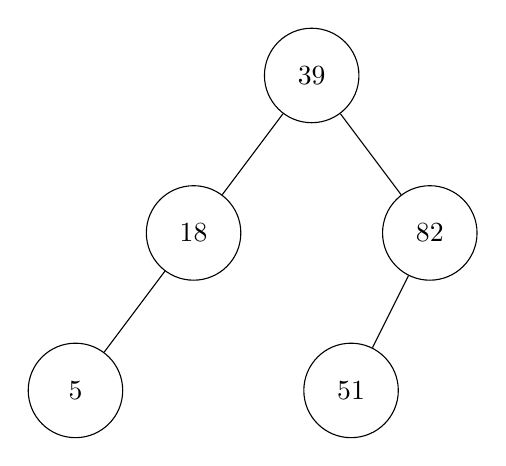
\begin{tikzpicture}
    \node[circle, draw, minimum size=1.2cm] (A) at (0, 0) {}; 
    \node[circle, draw, minimum size=1.2cm] (B) at (-1.5, -2) {};
    \node[circle, draw, minimum size=1.2cm] (C) at (-3, -4) {};
    \node[circle, draw, minimum size=1.2cm] (D) at (1.5, -2) {};
    \node[circle, draw, minimum size=1.2cm] (E) at (0.5, -4) {};

    % 線を引く
    \draw (A) --(B);
    \draw (B) -- (C);
    \draw (A) -- (D);
    \draw (D) -- (E);

    % 値を入れる
    \node at (0, 0) {39};
    \node at (-1.5, -2) {18};
    \node at (-3, -4) {5};
    \node at (1.5, -2) {82};
    \node at (0.5, -4) {51}; 

  \end{tikzpicture}
\end{center}

\subsection{二分木の実装}
\begin{lstlisting}[caption=二分木の実装, frame=TRBL, label={binary_tree}]
class Node:
  def __init__(self, data: int) -> None:
      self.data: int = data
      self.right: Node | None = None
      self.left: Node | None = None
      
  def __str__(self) -> str:
      return str(self.data)
  
class BinarySearchTree:
  def __init__(self):
      self.root = None
      
  def create(self, array: list[int]) -> None:
      for i in range(len(array)):
          self.insert(array[i])
  
  def insert(self, data: int) -> None:
      if self.root is None:
          self.root = Node(data)
      else:
          self._insert_recursively(self.root, data)
  
  def _insert_recursively(self, node: Node, data: int) -> None:
      if data <= node.data:
          if node.left is None:
              node.left = Node(data)
          else:
              self._insert_recursively(node.left, data)
      else:
          if node.right is None:
              node.right = Node(data)
          else:
              self._insert_recursively(node.right, data)
  
  def search(self, value: int) -> Node | None:
      if self.root is None:
          return self.root
      
      return self._search_recursively(self.root, value)
      
  def _search_recursively(self, node: Node, value: int) -> Node | None:
      if node.data == value:
          return node
      
      if value < node.data:
          if node.left is None:
              return node.left
          else:
              return self._search_recursively(node.left, value)
      else:
          if node.right is None:
              return node.right
          else:
              return self._search_recursively(node.right, value)
  
  def delete(self, value: int) -> Node | None:
      if self.root is None:
          return self.root
      else:
          self.root = self._delete_recursively(self.root, value)
  
  def _delete_recursively(self, node: Node, value: int) -> Node | None:
      if value < node.data:
          if node.left is None:
              return None
          else:
              node.left = self._delete_recursively(node.left, value)
      elif value > node.data:
          if node.right is None:
              return None
          else:
              node.right = self._delete_recursively(node.right, value)
      else:
          if node.left is None and node.right is None:
              return None
          elif node.left is None:
              return node.right
          elif node.right is None:
              return node.left
          else:
              successor = self._successor()
              node.data = successor.data
              self._delete_recursively(node.right, successor.data)
              
      return node
  
  def _successor(self) -> Node | None:
      if self.root is None:
          return self.root
      
      node = self.root
      
      while node.left is not None:
          node = node.left
      
      return node
\end{lstlisting}

\newpage

\section{平衡木}
\subsection{二分木の問題点}
二分木は最悪の場合木が以下のように片方に伸びてしまった場合、計算量が$O(n)$になってしまいます。

\vspace{0.5cm}

\begin{center}
  \begin{tikzpicture}[scale=0.6]
    \node[circle, draw, minimum size=1.2cm] (A) at (0, 0) {}; 
    \node[circle, draw, minimum size=1.2cm] (B) at (1.5, -2) {};
    \node[circle, draw, minimum size=1.2cm] (C) at (3, -4) {};
    \node[circle, draw, minimum size=1.2cm] (D) at (4.5, -6) {};
    \node[circle, draw, minimum size=1.2cm] (E) at (6, -8) {};

    % 線を引く
    \draw (A) --(B);
    \draw (B) -- (C);
    \draw (C) -- (D);
    \draw (D) -- (E);

    % 値を入れる
    \node at (0, 0) {1};
    \node at (1.5, -2) {2};
    \node at (3, -4) {3};
    \node at (4.5, -6) {4};
    \node at (6, -8) {5};

  \end{tikzpicture}
\end{center}

\vspace{0.5cm}

\subsection{平衡木}
平衡木は\textbf{回転}や乱択アルゴリズムを用いて木の高さを自動的に小さくする方向に調整できる木構造です。

扱う平衡木の代表的なものには以下のものがあります。

\begin{itemize}
  \item AVL木
  \item 赤黒木
  \item B木
  \item Treap
\end{itemize}

\subsection{AVL木}
AVL木とは、\textbf{Adelson-Velsky and Landis}の名前から取られた木構造で、以下の性質を持ちます。

\begin{itemize}
  \item 任意のノードにおいて、左右の部分木の高さの差が1以下である
\end{itemize}

\vspace{0.5cm}

以降の考察のために\textbf{balance factor}という言葉を導入します。

\begin{definitionbox}[balance factor]
  あるノードの左部分木の高さから右部分木の高さを引いた値を\textbf{balance factor}といいます。
  \begin{itemize}
    \item balance factor = 左部分木の高さ - 右部分木の高さ
  \end{itemize}
\end{definitionbox}

AVL木の性質をbalance factorを使って表すと以下のようになります。

\begin{itemize}
  \item 任意のノードにおいて、balance factorは-1, 0, 1のいずれかである
\end{itemize}

AVL木の例を以下に示します。ノードの横に書いてあるのがbalance factorです。

\vspace{0.5cm}

\begin{center}
  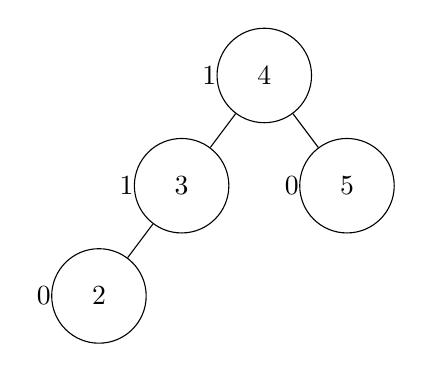
\begin{tikzpicture}[scale=0.7]
    \node[circle, draw, minimum size=1.2cm] (A) at (0, 0) {4}; 
    \node[circle, draw, minimum size=1.2cm] (B) at (-1.5, -2) {3};
    \node[circle, draw, minimum size=1.2cm] (C) at (-3, -4) {2};
    \node[circle, draw, minimum size=1.2cm] (E) at (1.5, -2) {5};


    % 線を引く
    \draw (A) --(B);
    \draw (B) -- (C);
    \draw (A) -- (E);

    % balance factor
    \node at (0 - 1, -1 + 1) {1};
    \node at (-1.5 - 1, -3 + 1) {1};
    \node at (-3 - 1, -5 + 1) {0};
    \node at (1.5 - 1, -3 + 1) {0};

  \end{tikzpicture}
\end{center}

次はAVL木の条件を満たしていない木です。
\vspace{0.5cm}

\begin{center}
  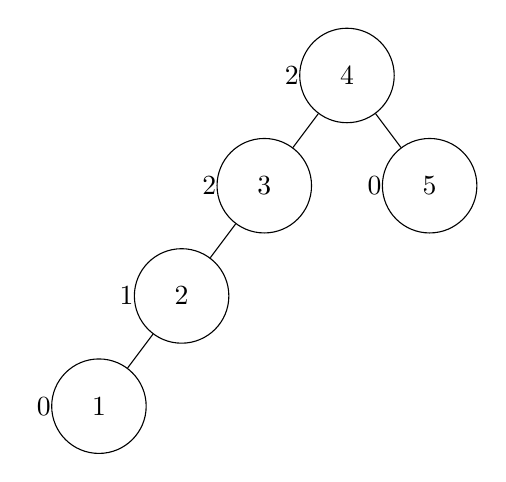
\begin{tikzpicture}[scale=0.7]
    \node[circle, draw, minimum size=1.2cm] (A) at (0, 0) {4}; 
    \node[circle, draw, minimum size=1.2cm] (B) at (-1.5, -2) {3};
    \node[circle, draw, minimum size=1.2cm] (C) at (-3, -4) {2};
    \node[circle, draw, minimum size=1.2cm] (D) at (-4.5, -6) {1};
    \node[circle, draw, minimum size=1.2cm] (E) at (1.5, -2) {5};


    % 線を引く
    \draw (A) --(B);
    \draw (B) -- (C);
    \draw (C) -- (D);
    \draw (A) -- (E);

    % balance factor
    \node at (0 - 1, -1 + 1) {2};
    \node at (-1.5 - 1, -3 + 1) {2};
    \node at (-3 - 1, -5 + 1) {1};
    \node at (-4.5 - 1, -7 + 1) {0};
    \node at (1.5 - 1, -3 + 1) {0};

  \end{tikzpicture}
\end{center}

\newpage

1. 左回転
\begin{center}
\begin{tikzpicture}[scale=0.7, every node/.style={circle, draw, minimum size=1.2cm}]
  \node (A) at (0, 2) {A}; 
  \node (B) at (2, 0) {B};
  \node (C) at (4, -2) {C};

  \draw (A) -- (B);
  \draw (B) -- (C);

  \node[draw=none, fill=none] at (7, 1) {$\longrightarrow$};
  \node[draw=none, fill=none] at (7, 2.5) {左回転};
  
  \node (B1) at (12, 2) {B}; 
  \node (A1) at (10, 0) {A};
  \node (C1) at (14, 0) {C};

  \draw (B1) -- (A1);
  \draw (B1) -- (C1);

  % balance factor
  \node[draw=none, fill=none] at (0, 2 + 1 + 0.2) {-2};
  \node[draw=none, fill=none] at (2, 0 + 1 + 0.2) {-1};
  \node[draw=none, fill=none] at (4, -2 + 1 + 0.2) {0};

  \node[draw=none, fill=none] at (12, 2 + 1 + 0.2) {0};
  \node[draw=none, fill=none] at (10, 0 + 1 + 0.2) {0};
  \node[draw=none, fill=none] at (14, 0 + 1 + 0.2) {0};
\end{tikzpicture}
\end{center}

2. 右回転
\begin{center}
  \begin{tikzpicture}[scale=0.7, every node/.style={circle, draw, minimum size=1.2cm}]    
    \node[draw=none, fill=none] at (6, 1) {$\longrightarrow$};
    \node[draw=none, fill=none] at (6, 2.5) {右回転};
    
    \node (C2) at (2, 2) {A}; 
    \node (B2) at (0, 0) {B};
    \node (A2) at (-2, -2) {C};
  
    \draw (C2) -- (B2);
    \draw (B2) -- (A2);
  
    \node (B3) at (12, 2) {B}; 
    \node (C3) at (10, 0) {C};
    \node (A3) at (14, 0) {A};

    \draw (B3) -- (C3);
    \draw (B3) -- (A3);

    % balance factor
    \node[draw=none, fill=none] at (2, 2 + 1 + 0.2) {2};
    \node[draw=none, fill=none] at (0, 0 + 1 + 0.2) {1};
    \node[draw=none, fill=none] at (-2, -2 + 1 + 0.2) {0};

    \node[draw=none, fill=none] at (12, 2 + 1 + 0.2) {0};
    \node[draw=none, fill=none] at (10, 0 + 1 + 0.2) {0};
    \node[draw=none, fill=none] at (14, 0 + 1 + 0.2) {0};
  \end{tikzpicture}
\end{center}

\vspace{0.5cm}

3. 左右回転
\begin{center}
  \begin{tikzpicture}[scale=0.7, every node/.style={circle, draw, minimum size=1.2cm}]    
    % 1個目の木 (Original Tree)
    \node (A) at (0, 2) {A}; 
    \node (C) at (-2, 0) {B};
    \node (B) at (0, -2) {C};

    \draw (A) -- (C);
    \draw (C) -- (B);

    % Arrow for Left Rotation
    \node[draw=none, fill=none] at (4, 1) {$\longrightarrow$};
    \node[draw=none, fill=none] at (4, 2.5) {左回転};
    
    % 2個目の木 (Intermediate Tree after Left Rotation)
    \node (A1) at (8, 2) {A}; 
    \node (B1) at (6, 0) {B};
    \node (C1) at (4, -2) {C};

    \draw (A1) -- (B1);
    \draw (B1) -- (C1);

    % Arrow for Right Rotation
    \node[draw=none, fill=none] at (12, 1) {$\longrightarrow$};
    \node[draw=none, fill=none] at (12, 2.5) {右回転};
    
    % 3個目の木 (Final Balanced Tree after Right Rotation)
    \node (B2) at (16, 2) {A}; 
    \node (A2) at (14, 0) {B};
    \node (C2) at (18, 0) {C};

    % Drawing the edges
    \draw (B2) -- (A2);
    \draw (B2) -- (C2);

    % balance factor
    \node[draw=none, fill=none] at (0, 2 + 1 + 0.2) {2};
    \node[draw=none, fill=none] at (-2, 0 + 1 + 0.2) {-1};
    \node[draw=none, fill=none] at (0, -2 + 1 + 0.2) {0};

    \node[draw=none, fill=none] at (8, 2 + 1 + 0.2) {2};
    \node[draw=none, fill=none] at (6, 0 + 1 + 0.2) {1};
    \node[draw=none, fill=none] at (4, -2 + 1 + 0.2) {0};

    \node[draw=none, fill=none] at (16, 2 + 1 + 0.2) {0};
    \node[draw=none, fill=none] at (14, 0 + 1 + 0.2) {0};
    \node[draw=none, fill=none] at (18, 0 + 1 + 0.2) {0};
  \end{tikzpicture}
\end{center}

4. 右左回転

\begin{center}
  \begin{tikzpicture}[scale=0.7, every node/.style={circle, draw, minimum size=1.2cm}]    
    % 1個目の木 (Original Tree)
    \node (A) at (0, 2) {A}; 
    \node (B) at (2, 0) {B};
    \node (C) at (0, -2) {C};

    \draw (A) -- (B);
    \draw (B) -- (C);

    % Arrow for Right Rotation
    \node[draw=none, fill=none] at (6, 1) {$\longrightarrow$};
    \node[draw=none, fill=none] at (6, 2.5) {右回転};
    
    % 2個目の木 (Intermediate Tree after Right Rotation)
    \node (B1) at (10, 2) {B}; 
    \node (A1) at (12, 0) {A};
    \node (C1) at (14, -2) {C};

    \draw (B1) -- (A1);
    \draw (A1) -- (C1);

    % Arrow for Left Rotation
    \node[draw=none, fill=none] at (16, 1) {$\longrightarrow$};
    \node[draw=none, fill=none] at (16, 2.5) {左回転};
    
    % 3個目の木 (Final Balanced Tree after Left Rotation)
    \node (B2) at (20, 2) {B}; 
    \node (A2) at (18, 0) {A};
    \node (C2) at (22, 0) {C};

    % Drawing the edges
    \draw (B2) -- (A2);
    \draw (B2) -- (C2);

    % balance factor
    \node[draw=none, fill=none] at (0, 2 + 1 + 0.2) {-2};
    \node[draw=none, fill=none] at (2, 0 + 1 + 0.2) {1};
    \node[draw=none, fill=none] at (0, -2 + 1 + 0.2) {0};

    \node[draw=none, fill=none] at (10, 2 + 1 + 0.2) {-2};
    \node[draw=none, fill=none] at (12, 0 + 1 + 0.2) {-1};
    \node[draw=none, fill=none] at (14, -2 + 1 + 0.2) {0};

    \node[draw=none, fill=none] at (20, 2 + 1 + 0.2) {0};
    \node[draw=none, fill=none] at (18, 0 + 1 + 0.2) {0};
    \node[draw=none, fill=none] at (22, 0 + 1 + 0.2) {0};
  \end{tikzpicture}
\end{center}

  \begin{lstlisting}[caption=二分ヒープの実装, label=binaryheap, frame=TRBL, label={binaryheap}]
  class Node:
      def \_\_init\_\_(self, value: int) -> None:
          self.data: int = value
          self.left: Node | None = None
          self.right: Node | None = None
          self.height: int = 0
      
      def \_\_str\_\_(self) -> str:
          return f"Node: data = {self.data} height = {self.height}"
          
  class AVLTree:
      def \_\_init\_\_(self):
          self.root = None
      
      def \_height(self, node: Node | None) -> int:
          if node is None:
              return -1
          
          return node.height
          
      def \_update\_height(self, node:
       Node) -> None:
          node.height = 1 + max(self.\_height(node.left), self.\_height(node.right))
  
      def \_balance\_factor(self, node: Node) -> int:
          return self.\_height(node.left) - self.\_height(node.right)
  
      def \_right\_rotate(self, node: Node) -> Node:
          new\_root = node.left
          node.left = new\_root.right
          new\_root.right = node
          
          self.\_update\_height(node)
          self.\_update\_height(new\_root)
          
          return new\_root 
      
      def \_left\_rotate(self, node: Node) -> Node:
          new\_root = node.right
          node.right = new\_root.left
          new\_root.left = node
          
          self.\_update\_height(node)
          self.\_update\_height(new\_root)
          
          return new\_root
          
      def create(self, values: list[int]) -> None:
          for value in values:
              self.insert(value)
      
      def insert(self, value: int) -> None:
          if self.root is None:
              self.root = Node(value)
              return self.root
          else:
              self.root = self.\_insert\_recursively(self.root, value)
              return self.root
      
      def \_insert\_recursively(self, node: Node, value: int) -> Node:
          if value <= node.data:
              if node.left is None:
                  node.left = Node(value)
              else:
                  node.left = self.\_insert\_recursively(node.left, value)
          else:
              if node.right is None:
                  node.right = Node(value)
              else:
                  node.right = self.\_insert\_recursively(node.right, value)
          
          self.\_update\_height(node)
          
          balance\_factor = self.\_balance\_factor(node)
          
          if balance\_factor > 1 and value < node.left.data:
              return self.\_right\_rotate(node)
          
          if balance\_factor > 1 and value > node.left.data:
              node.left = self.\_left\_rotate(node.left)
              return self.\_right\_rotate(node)
          
          if balance\_factor < -1 and value > node.right.data:
              return self.\_left\_rotate(node)
          
          if balance\_factor < -1 and value < node.right.data:
              node.right = self.\_right\_rotate(node.right)
              return self.\_left\_rotate(node)
          
          return node
          
      
      def search(self, value: int) -> Node | None:
          if self.root is None:
              return None
          
          return self.\_search\_recursively(self.root, value)
  
      def \_search\_recursively(self, node: Node, value: int) -> Node | None:
          if value == node.data:
              return node
          
          if value < node.data:
              if node.left is None:
                  return None
              else:
                  return self.\_search\_recursively(node.left, value)
          else:
              if node.right is None:
                  return None
              else:
                  return self.\_search\_recursively(node.right, value)
              
      
      def delete(self, value: int) -> Node | None:
          if self.root is None:
              return self.root
          else:
              self.root = self.\_delete\_recursively(self.root, value)
              return self.root
      
      def \_delete\_recursively(self, node: Node, value: int) -> Node | None:
          if value < node.data:
              node.left = self.\_delete\_recursively(node.left, value)
          elif value > node.data:
              node.right = self.\_delete\_recursively(node.right, value)
          else:
              if node.left is None and node.right is None:
                  return None
              elif node.left is None:
                  return node.right
              elif node.right is None:
                  return node.left
              else:
                  min\_node = self.\_find\_min(node.right)
                  node.data = min\_node.data
                  node.right = self.\_delete\_recursively(node.right, min\_node.data)
          
          self\.\_update\_height(node)
          
          balance\_factor = self.\_balance\_factor(node)
          
          if balance\_factor > 1 and self.\_balance\_factor(node.left) >= 0:
              return self.\_right\_rotate(node)
          
          if balance\_factor < -1 and self.\_balance\_factor(node.right) <= 0:
              return self.\_left\_rotate(node)
          
          if balance\_factor > 1 and self.\_balance\_factor(node.left) < 0:
              node.left = self.\_left\_rotate(node.left)
              return self.\_right\_rotate(node)
          
          if balance\_factor < -1 and self.\_balance\_factor(node.right) > 0:
              node.right = self.\_right\_rotate(node.right)
              return self.\_left\_rotate(node)
          
          return node
  \end{lstlisting}

\newpage
\subsection{B木}
AVL木は二分木であるため、データの数が多い場合に気が高くなり検索や挿入に時間がかかってしまう問題があります。そこで枝の数が
2本よりも多く取るB木というデータ構造を紹介します。B木は応用範囲が広く以下の様な様々なものに使われています。

\begin{itemize}
  \item データベース
  \item ファイルシステム
\end{itemize}

B木はノードが持てる最大の枝の本数$order$によって定義されます。二分木ではノードは1つの値を持っていてその値との大小比較で
左右の子ノードに振り分けていましたが、B木ではノードが複数の値を持ち、その値の範囲で子ノードに振り分けます。
order=$3$のB木の例を以下に示します。\texttt{[10, 5, 3, 2, 8, 4, 1, 6]}
のデータをorder=$3$のB木に入れていきます。

\vspace{0.5cm}

\begin{center}
  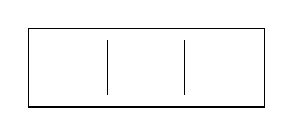
\begin{tikzpicture}[scale=0.7, every node/.style={circle, draw, minimum size=1.2cm}]    
    \node [rectangle, minimum width=3cm, minimum height=1cm, draw] (A) at (0, 0) {};
    \draw (0.7, 0.5) -- (0.7, -0.5);
    \draw (-0.7, 0.5) -- (-0.7, -0.5);
  \end{tikzpicture}
\end{center}

\subsubsection{B木の実装}

\begin{lstlisting}[caption=B木の実装, label=btree, frame=TRBL, label={btree}]
from bisect import bisect_left, bisect_right

class Node:
    def __init__(self):
        self.keys: list[int] = []
        self.children: list[Node] = []

class BTree:
    def __init__(self, order: int) -> None:
        self.order = order
        self.root = Node()
    
    def _median(self, array: list[int]) -> int:
        return array[len(array) // 2]

    def insert(self, value: int) -> None:
        node = self._insert_recursively(self.root, value)
        if node:
            new_root = Node()
            new_root.keys = [node[0]]
            new_root.children = [node[1], node[2]]
            self.root = new_root
    
    def _insert_recursively(self, node: Node, value: int):
        # 葉ノード
        if not node.children:
            node.keys.append(value)
            node.keys.sort()
            if len(node.keys) < self.order:
                return None 
            else:
                return self._split(node)
        else:  
            index = bisect_right(node.keys, value)
            result = self._insert_recursively(node.children[index], value)
            
            if result is not None:
                median, left_node, right_node = result
                node.keys.insert(index, median)
                
                # 修正:左ノードを適切に設定し、右ノードを挿入
                node.children[index] = left_node  # 左の子ノードを置き換える
                node.children.insert(index + 1, right_node)  # 右の子ノードを挿入

                if len(node.keys) < self.order:
                    return None
                else:
                    return self._split(node) 
            return None

    def _split(self, node: Node):
        median_index = len(node.keys) // 2
        median = node.keys[median_index]

        left_node = Node()
        right_node = Node()

        left_node.keys = node.keys[:median_index]
        right_node.keys = node.keys[median_index + 1:]

        if node.children:
            left_node.children = node.children[:median_index + 1]
            right_node.children = node.children[median_index + 1:]

        return median, left_node, right_node

    def search(self, value: int) -> bool:
        node = self.root
        if value in node.keys:
            return True
        else:
            return self._search_recursively(self.root, value)
    
    def _search_recursively(self, node: Node, value: int) -> bool:
        if len(node.children) == 0:
            return False
        
        index = bisect_left(node.keys, value)
        next_node = node.children[index]
        
        if value in next_node.keys:
            return True
        else:
            return self._search_recursively(node.children[index], value)

b_tree = BTree(order=3)
b_tree.insert(5)
b_tree.insert(10)
b_tree.insert(15)
b_tree.insert(20)
b_tree.insert(30)

b_tree.insert(21)
b_tree.insert(22)
\end{lstlisting}

\newpage

\subsection{赤黒木}
赤黒木はAVL木同様平衡二分探索木の1つで、以下の特徴を持っています。

\begin{itemize}
  \item 各ノードは赤か黒の色を持つ
  \item 根ノードは黒である
  \item 赤のノードの子ノードは黒である
  \item あるノードからその子孫の葉ノードまでの黒の数は同じである
  \item 葉ノードは黒である
\end{itemize}


\section{参考}
\textbf{二分探索}

\begin{itemize}
  \item \url{https://qiita.com/drken/items/97e37dd6143e33a64c8c}
\end{itemize}


\noindent \textbf{二分探索木}
\begin{itemize}
  \item \url{https://www.geeksforgeeks.org/introduction-to-avl-tree/}
\end{itemize}

\noindent \textbf{B木}
\begin{itemize}
  \item \url{https://www.geeksforgeeks.org/b-tree-in-python/}
  \item \url{https://www.javatpoint.com/b-tree}
  \item \url{https://wqwq3215.medium.com/b-tree%E3%82%92%E7%90%86%E8%A7%A3%E3%81%97%E3%81%A6%E3%81%84%E3%81%8F-142f93fc3c6c}
\end{itemize}

\noindent \textbf{赤黒木}

\begin{itemize}
  \item \url{https://qiita.com/kgoto/items/b15b9a494deae010d660}
  \item \url{http://wwwa.pikara.ne.jp/okojisan/rb-tree/index.html}
\end{itemize}